\RequirePackage{luatex85}
\documentclass[tikz]{standalone}
% Default preamble
\usepackage{pgfplots}
\pgfplotsset{compat=newest}
\usepgfplotslibrary{groupplots}
\usepgfplotslibrary{polar}
\usepgfplotslibrary{smithchart}
\usepgfplotslibrary{statistics}
\usepgfplotslibrary{dateplot}
\usepgfplotslibrary{ternary}
\usetikzlibrary{arrows.meta}
\usetikzlibrary{backgrounds}
\usepgfplotslibrary{patchplots}
\usepgfplotslibrary{fillbetween}
\pgfplotsset{%
layers/standard/.define layer set={%
    background,axis background,axis grid,axis ticks,axis lines,axis tick labels,pre main,main,axis descriptions,axis foreground%
}{grid style= {/pgfplots/on layer=axis grid},%
    tick style= {/pgfplots/on layer=axis ticks},%
    axis line style= {/pgfplots/on layer=axis lines},%
    label style= {/pgfplots/on layer=axis descriptions},%
    legend style= {/pgfplots/on layer=axis descriptions},%
    title style= {/pgfplots/on layer=axis descriptions},%
    colorbar style= {/pgfplots/on layer=axis descriptions},%
    ticklabel style= {/pgfplots/on layer=axis tick labels},%
    axis background@ style={/pgfplots/on layer=axis background},%
    3d box foreground style={/pgfplots/on layer=axis foreground},%
    },
}

\begin{document}
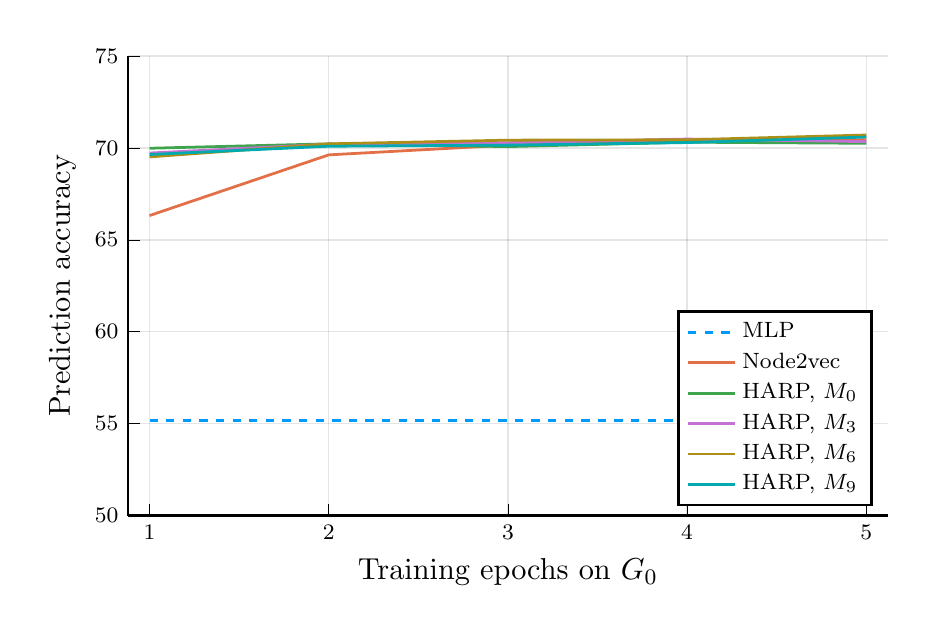
\begin{tikzpicture}[/tikz/background rectangle/.style={fill={rgb,1:red,1.0;green,1.0;blue,1.0}, draw opacity={1.0}}, show background rectangle]
\begin{axis}[point meta max={nan}, point meta min={nan}, legend cell align={left}, title={}, title style={at={{(0.5,1)}}, anchor={south}, font={{\fontsize{14 pt}{18.2 pt}\selectfont}}, color={rgb,1:red,0.0;green,0.0;blue,0.0}, draw opacity={1.0}, rotate={0.0}}, legend style={color={rgb,1:red,0.0;green,0.0;blue,0.0}, draw opacity={1.0}, line width={1}, solid, fill={rgb,1:red,1.0;green,1.0;blue,1.0}, fill opacity={1.0}, text opacity={1.0}, font={{\fontsize{8 pt}{10.4 pt}\selectfont}}, text={rgb,1:red,0.0;green,0.0;blue,0.0}, at={(0.98, 0.02)}, anchor={south east}}, axis background/.style={fill={rgb,1:red,1.0;green,1.0;blue,1.0}, opacity={1.0}}, anchor={north west}, xshift={1.0mm}, yshift={-1.0mm}, width={112.3mm}, height={74.2mm}, scaled x ticks={false}, xlabel={Training epochs on $G_0$}, x tick style={color={rgb,1:red,0.0;green,0.0;blue,0.0}, opacity={1.0}}, x tick label style={color={rgb,1:red,0.0;green,0.0;blue,0.0}, opacity={1.0}, rotate={0}}, xlabel style={at={(ticklabel cs:0.5)}, anchor=near ticklabel, font={{\fontsize{11 pt}{14.3 pt}\selectfont}}, color={rgb,1:red,0.0;green,0.0;blue,0.0}, draw opacity={1.0}, rotate={0.0}}, xmajorgrids={true}, xmin={0.88}, xmax={5.12}, xtick={{1.0,2.0,3.0,4.0,5.0}}, xticklabels={{$1$,$2$,$3$,$4$,$5$}}, xtick align={inside}, xticklabel style={font={{\fontsize{8 pt}{10.4 pt}\selectfont}}, color={rgb,1:red,0.0;green,0.0;blue,0.0}, draw opacity={1.0}, rotate={0.0}}, x grid style={color={rgb,1:red,0.0;green,0.0;blue,0.0}, draw opacity={0.1}, line width={0.5}, solid}, axis x line*={left}, x axis line style={color={rgb,1:red,0.0;green,0.0;blue,0.0}, draw opacity={1.0}, line width={1}, solid}, scaled y ticks={false}, ylabel={Prediction accuracy}, y tick style={color={rgb,1:red,0.0;green,0.0;blue,0.0}, opacity={1.0}}, y tick label style={color={rgb,1:red,0.0;green,0.0;blue,0.0}, opacity={1.0}, rotate={0}}, ylabel style={at={(ticklabel cs:0.5)}, anchor=near ticklabel, font={{\fontsize{11 pt}{14.3 pt}\selectfont}}, color={rgb,1:red,0.0;green,0.0;blue,0.0}, draw opacity={1.0}, rotate={0.0}}, ymajorgrids={true}, ymin={50}, ymax={75}, ytick={{50.0,55.0,60.0,65.0,70.0,75.0}}, yticklabels={{$50$,$55$,$60$,$65$,$70$,$75$}}, ytick align={inside}, yticklabel style={font={{\fontsize{8 pt}{10.4 pt}\selectfont}}, color={rgb,1:red,0.0;green,0.0;blue,0.0}, draw opacity={1.0}, rotate={0.0}}, y grid style={color={rgb,1:red,0.0;green,0.0;blue,0.0}, draw opacity={0.1}, line width={0.5}, solid}, axis y line*={left}, y axis line style={color={rgb,1:red,0.0;green,0.0;blue,0.0}, draw opacity={1.0}, line width={1}, solid}, colorbar={false}]
    \addplot[color={rgb,1:red,0.0;green,0.6056;blue,0.9787}, name path={0505f456-c5c3-4b6f-850e-ee386615a912}, draw opacity={1.0}, line width={1}, dashed]
        table[row sep={\\}]
        {
            \\
            1.0  55.189998626708984  \\
            5.0  55.189998626708984  \\
        }
        ;
    \addlegendentry {MLP}
    \addplot[color={rgb,1:red,0.8889;green,0.4356;blue,0.2781}, name path={98d257ac-226b-4462-9e8d-2fb41fc3dd27}, draw opacity={1.0}, line width={1}, solid]
        table[row sep={\\}]
        {
            \\
            1.0  66.32  \\
            2.0  69.62  \\
            3.0  70.15  \\
            4.0  70.39  \\
            5.0  70.44  \\
        }
        ;
    \addlegendentry {Node2vec}
    \addplot[color={rgb,1:red,0.2422;green,0.6433;blue,0.3044}, name path={2c5cf957-8034-484c-bfb1-7ea6ae0bcfc9}, draw opacity={1.0}, line width={1}, solid]
        table[row sep={\\}]
        {
            \\
            1.0  69.98  \\
            2.0  70.22  \\
            3.0  70.07  \\
            4.0  70.31  \\
            5.0  70.25  \\
        }
        ;
    \addlegendentry {HARP, $M_0$}
    \addplot[color={rgb,1:red,0.7644;green,0.4441;blue,0.8243}, name path={7439b959-3b53-4899-a31f-1349e7aed219}, draw opacity={1.0}, line width={1}, solid]
        table[row sep={\\}]
        {
            \\
            1.0  69.72  \\
            2.0  70.2  \\
            3.0  70.28  \\
            4.0  70.48  \\
            5.0  70.34  \\
        }
        ;
    \addlegendentry {HARP, $M_3$}
    \addplot[color={rgb,1:red,0.6755;green,0.5557;blue,0.0942}, name path={43aa9f77-5f38-4e29-a62e-0863ec3c59c7}, draw opacity={1.0}, line width={1}, solid]
        table[row sep={\\}]
        {
            \\
            1.0  69.51  \\
            2.0  70.22  \\
            3.0  70.42  \\
            4.0  70.44  \\
            5.0  70.7  \\
        }
        ;
    \addlegendentry {HARP, $M_6$}
    \addplot[color={rgb,1:red,0.0;green,0.6658;blue,0.681}, name path={4f5d8b83-b273-4368-9241-317cc1946836}, draw opacity={1.0}, line width={1}, solid]
        table[row sep={\\}]
        {
            \\
            1.0  69.64  \\
            2.0  70.09  \\
            3.0  70.15  \\
            4.0  70.29  \\
            5.0  70.59  \\
        }
        ;
    \addlegendentry {HARP, $M_9$}
\end{axis}
\end{tikzpicture}
\end{document}
